\section{Příklad 3E -- Pravděpodobnost bezporuchového provozu}



V klínových řemenech byla zjištěna následující provozní napětí $\sigma_p$ v MPa:

\[
\sigma_p =
\{223;\ 116;\ 158{,}5;\ 199;\ 136{,}5;\ 169{,}5;\ 267{,}5;\ 127;\ 184;\ 151\}
\]


\noindent
Dále byly zjištěny následující hodnoty meze pevnosti $R_m$ v MPa:

\[
R_m =
\{211;\ 269{,}5;\ 192;\ 301{,}5;\ 220{,}5;\ 243{,}5;\ 182{,}5;\ 257;\ 234;\ 199{,}5;\ 216;\ 205\}
\]

Cílem výpočtu je stanovit pravděpodobnost bezporuchového provozu ve tvaru:

\begin{equation}
P_{\text{bezp.}} = P(R_m > \sigma_p)
\label{eq:pravd}
\end{equation}

\subsection*{Předpoklad výpočtu}

Obě veličiny byly uvažovány jako náhodné s normálním rozdělením:

\begin{equation}
\sigma_p \sim \mathcal{N}(\mu_{\sigma}, s_{\sigma}), \qquad
R_m \sim \mathcal{N}(\mu_R, s_R)
\label{eq:normalita}
\end{equation}


\noindent
Z dat byly stanoveny statistické charakteristiky:

\[
\mu_{\sigma} = 173{,}20\ \text{MPa}, \quad
s_{\sigma} = 46{,}70\ \text{MPa}
\]

\[
\mu_R = 227{,}67\ \text{MPa}, \quad
s_R = 34{,}95\ \text{MPa}
\]

\subsection*{Kontrola normality}

Pro ověření předpokladu normálního rozdělení byla zvolena hladina významnosti:
\[
\alpha = 0{,}05
\]
Při této hladině významnosti se rozhoduje o zamítnutí nulové hypotézy na základě~p-~hodnoty.

Dále byl použit Lillieforsův test, který je modifikací Kolmogorov--Smirnovova testu a je vhodný v případech, kdy parametry normálního rozdělení nejsou předem známy, ale jsou odhadovány z dat. Tento test je v prostředí MATLAB implementován přímo pomocí funkce \texttt{lillietest}, která umožňuje automatický výpočet testovací statistiky i p-hodnoty.

Normalita dat byla současně ověřena i vizuálně pomocí Q-Q diagramu (obr.~\ref{fig:qq_plot}).

\begin{figure}[H]
    \centering
    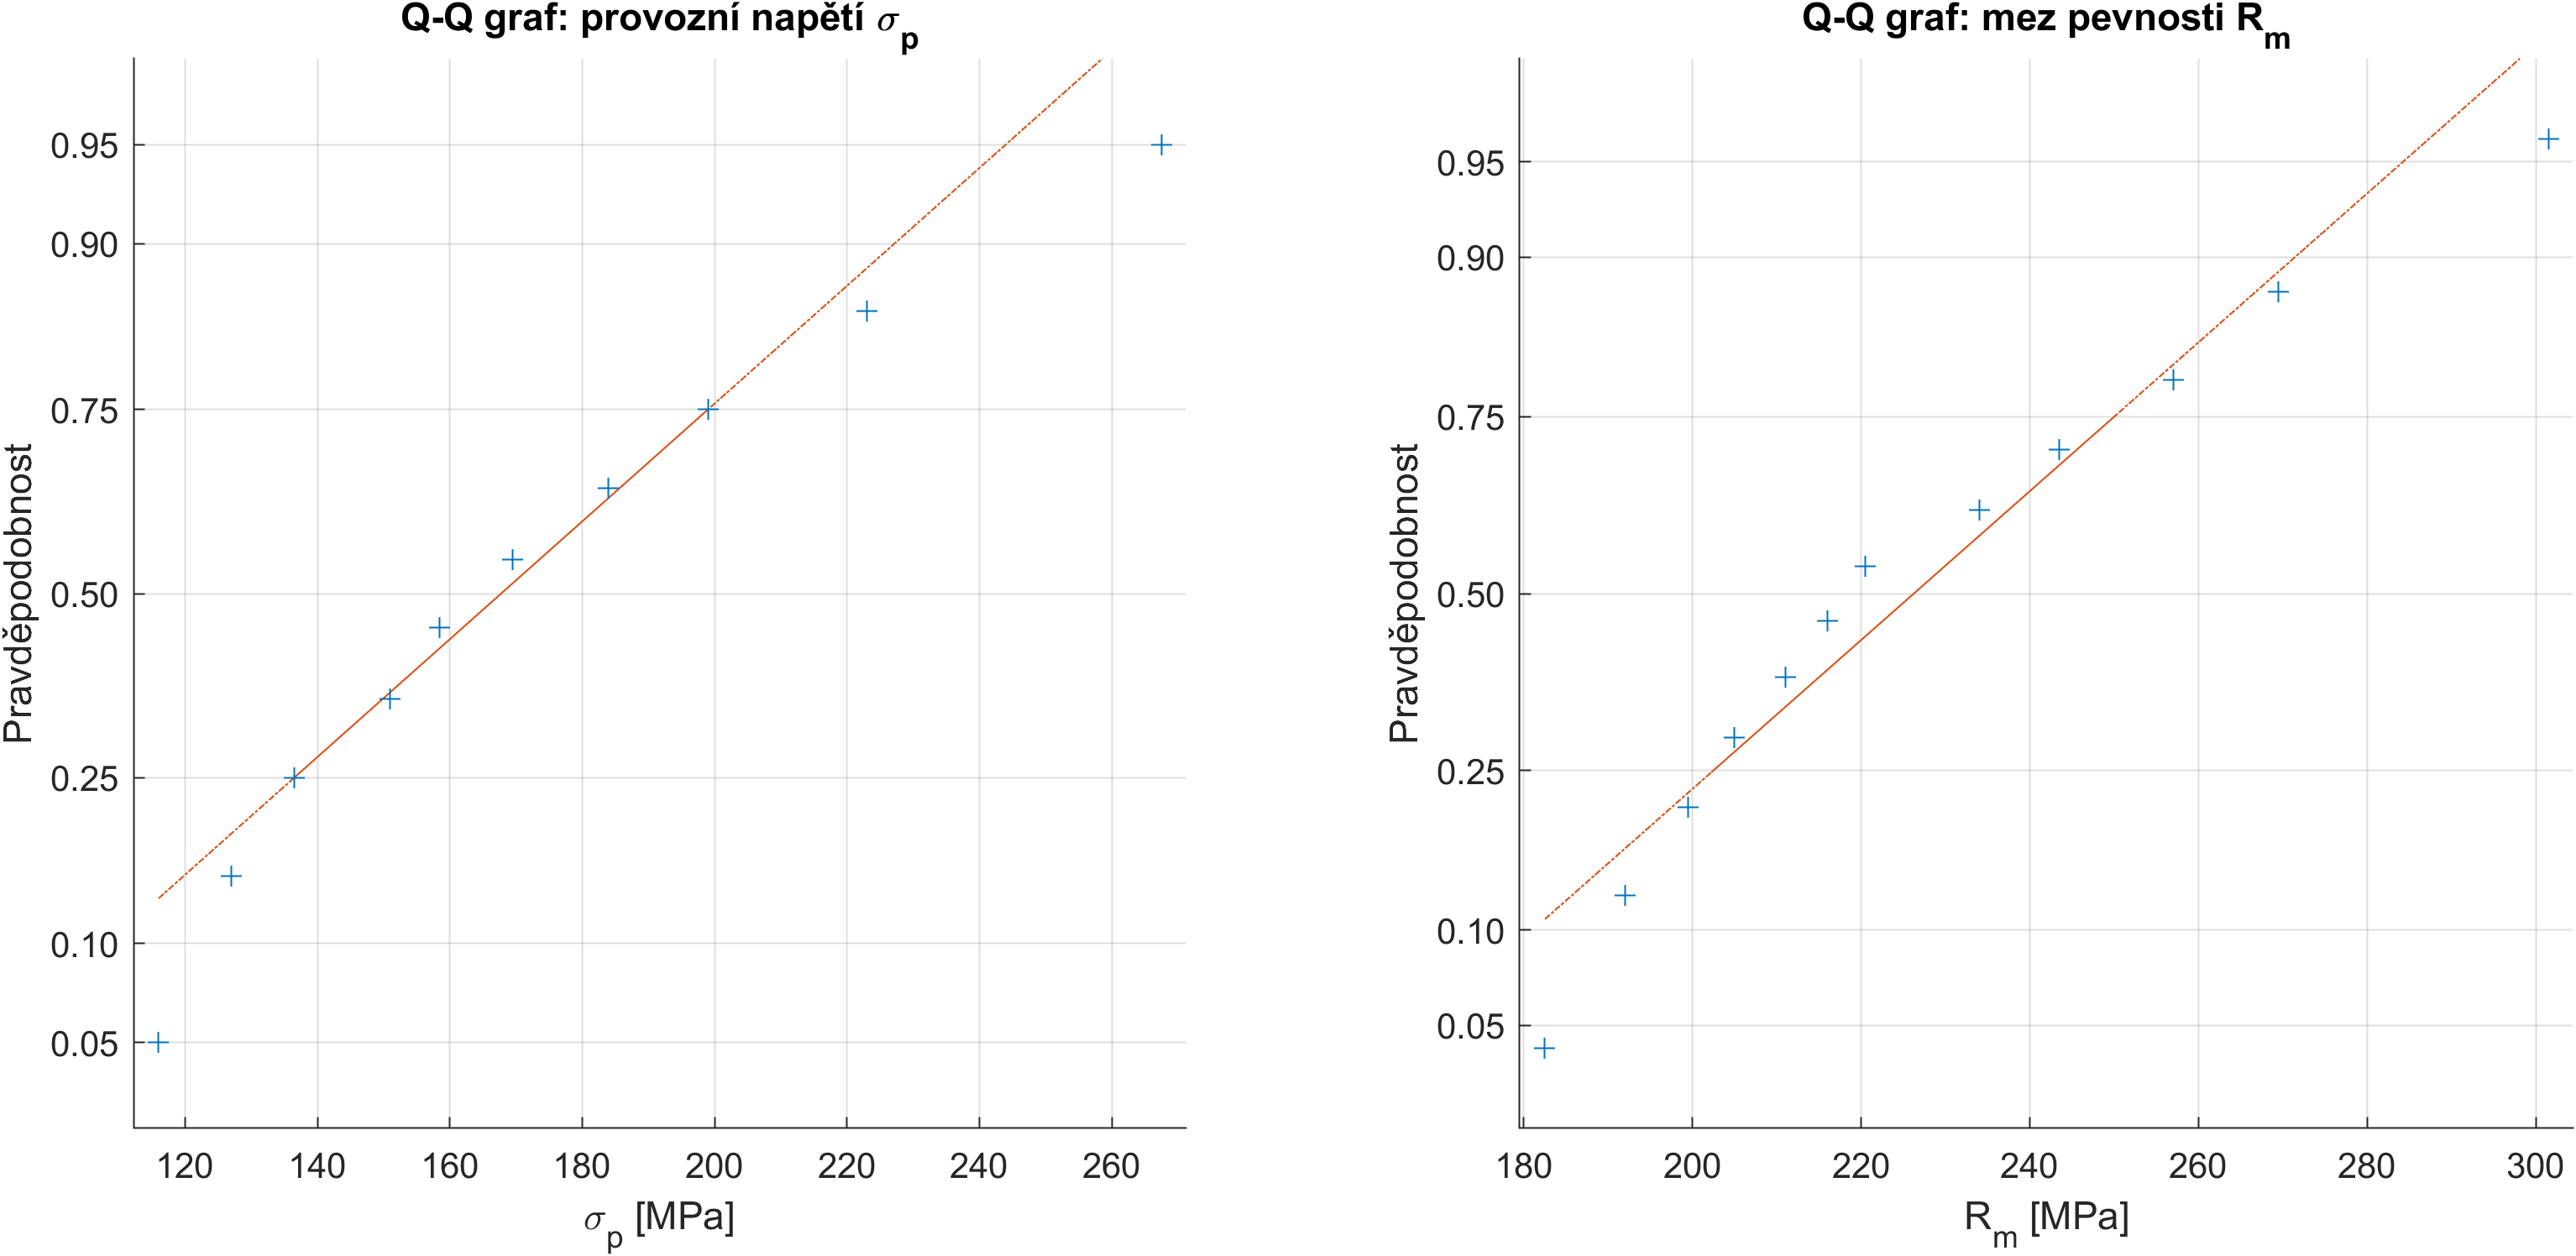
\includegraphics[width=0.95\textwidth]{qq_grafy.png}
    \caption{Q-Q diagram pro provozní napětí $\sigma_p$ a mez pevnosti $R_m$}
    \label{fig:qq_plot}
\end{figure}

Výsledky testu:

\[
p_{\sigma_p} = 0{,}5000, \qquad p_{R_m} = 0{,}4792
\]

\noindent
Protože v obou případech platí $p > \alpha = 0{,}05$, nelze zamítnout nulovou hypotézu o normálním rozdělení.  
Předpoklad uvedený ve vztahu~(\ref{eq:normalita}) je tedy pro další výpočet přijatelný.

\subsection*{Výpočet indexu spolehlivosti}

Zavedeme rozdílovou veličinu:

\begin{equation}
Z = R_m - \sigma_p
\label{eq:Z}
\end{equation}

\noindent
Bezporuchový provoz nastává, pokud $Z > 0$. Index spolehlivosti je definován jako:

\begin{equation}
\beta =
\frac{\mu_R - \mu_{\sigma}}
{\sqrt{s_R^2 + s_{\sigma}^2}}
\label{eq:beta}
\end{equation}

Po dosazení:

\[
\beta =
\frac{227{,}67 - 173{,}20}
{\sqrt{34{,}95^2 + 46{,}70^2}}
= 0{,}9337
\]

\subsection*{Výpočet pravděpodobnosti}

Hledaná pravděpodobnost ze vztahu~(\ref{eq:pravd}) se určí pomocí distribuční funkce normálního rozdělení:

\begin{equation}
P_{\text{bezp.}} = \Phi(\beta)
\label{eq:Phi}
\end{equation}

Po dosazení:

\[
P_{\text{bezp.}} = \Phi(0{,}9337) = 0{,}8248
\]

\[
P_{\text{bezp.}} = 82{,}48 \%
\]

\subsection*{Závěr}

Na základě provedeného výpočtu byla pravděpodobnost bezporuchového provozu stanovena jako:

\[
\boxed{P_{\text{bezp.}} = 0{,}8248 \approx 82{,}48\,\%}
\]

\noindent
Pravděpodobnost poruchy je:

\[
\boxed{P_{\text{por.}} = 0{,}1752 \approx 17{,}52\,\%}
\]

\noindent
Při uvažovaném normálním rozdělení veličin $\sigma_p$ a $R_m$ je tedy pravděpodobnost bezporuchového provozu přibližně $82{,}5\,\%$.

